
\chapter{Problem Solving}

\fellow{Formatting: can we put things marked ``Problem'' in a box (maybe with some color?) to set it apart?  Same with the Think/Pair/Share (different color?) and Solutions.}

\begin{problem}[ABC]
Draw curves connecting A to A, B to B, and C to C.  Your curves can't cross or even touch each other, and they can't go outside the box.
\begin{center}
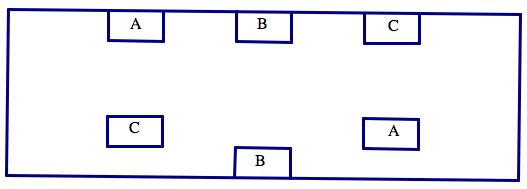
\includegraphics[height=4 cm]{prob1_pic1}
\end{center}
\end{problem}


\begin{thinkpair*}
After you have worked on the problem on your own for a while, talk through your ideas with a partner (even if you haven't solved it).  What did you try?   What makes this problem difficult?  Can you change the problem slightly so that it would be easier to solve?
\end{thinkpair*}

\begin{ps}[Wishful Thinking]
Don't you \emph{\bf wish} the picture in the problem looked more like this one?  Could you solve the problem in that case?
\begin{center}
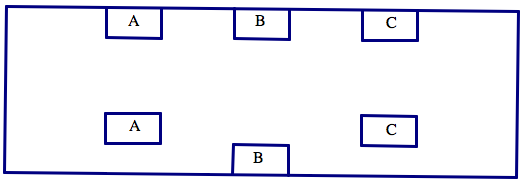
\includegraphics[height=4 cm]{prob1_pic2}
\end{center}
\end{ps}

Can you use a solution to this easier problem to help you solve the original problem?  How?  Think about moving the boxes around once the lines are already drawn.

\fellow{Would be great to have an animation here showing how one solution transforms into the other.  Not sure how hard that would be to create...}

The Common Core State Standards for Mathematics (\url{http://www.corestandards.org/Math/Practice}) identify eight ``Mathematical Practices'' --- the kinds of expertise that all teachers should try to foster in their students, but that go far beyond any particular piece of mathematics content.  They describe what mathematics is really about, and why it is so valuable for students to master.  The very first Mathematical Practice is:

\begin{quote}
``{\bf Make sense of problems and persevere in solving them.}\\
Mathematically proficient students start by explaining to themselves the meaning of a problem and looking for entry points to its solution. They analyze givens, constraints, relationships, and goals. They make conjectures about the form and meaning of the solution and plan a solution pathway rather than simply jumping into a solution attempt. They consider analogous problems, and try special cases and simpler forms of the original problem in order to gain insight into its solution. They monitor and evaluate their progress and change course if necessary.''
\end{quote}

This chapter will help you develop these very important mathematical skills, so that you'll be better prepared to help your future students develop them.


\section{Problem or Exercise?}
The main activity of mathematics is {\bf solving problems}.  But what most people experience in most mathematics classrooms is {\bf practice exercises}.  An exercise is different from a problem.


In a {\bf problem}, you probably don't know at first how to approach solving it.  You 
don't know what mathematical ideas might be used in the solution.  Part of solving a problem is understanding what is being asked, and knowing what a solution should even look like.  Problems often involve false starts, making mistakes, and lots of scratch paper!

In an {\bf exercise}, you are often practicing a skill.  You may have seen a teacher demonstrate a technique, or you may have read a worked example in the book.  You then \emph{practice} on very similar problems, with the goal of mastering that skill.


Note: What is a {\bf problem} for some people may be an {\bf exercise} for other people who have more background knowledge!  For a young student just learning addition, this might be a problem:  
\begin{center}
\emph{Fill in the blank to make a true statement: $\underline{\qquad} + 4 = 7$. }
\end{center}
But for you, that is an exercise!

Both problems and exercises are important in mathematics learning.  But we should never forget that the ultimate goal is to develop more and better skills (through exercises) so that we can solve harder and more interesting problems.  

Learning math is a bit like learning to play a sport.  You can practice lots of skills --- hitting hundreds of forehands in tennis so that you can place them in a particular spot in the court, breaking down strokes into the component pieces in swimming so that each part of the stroke is more efficient, keeping control of the ball while making quick turns in soccer, shooting free throws in basketball, catching high fly balls in baseball, and so on --- but the whole point of the sport is to \emph{play the game}.  You practice the skills so that you're better at playing the game!

The game of math, that's solving problems!

\subsection*{On Your Own}
For each question below, decide if it is a {\bf problem} or an {\bf exercise}.   (You do not need to solve the problems!  Just decide which category it fits for you.)  After you have labeled each one, compare your answers with a partner.

\fellow{Add a mix of exercises.  Use the problems provided here.  Throw in some straightforward computations like adding fractions with unlike denominators, multiplying two-digit numbers, and solving some linear equations.  Make a couple of them ``word problems'' but exercise-y ones like: ``What number is 3 more than 20?''  You can just flip through the book.  Choose about six or seven exercises to go with the problems shows, and intersperse them.}

\begin{enumerate}

\item
 This clock has been broken into three pieces.  If you add the numbers in each piece, the sums are consecutive numbers.  Can you break another clock into a different number of pieces so that the sums are consecutive numbers?  
\begin{center}
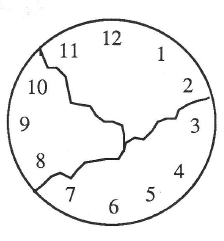
\includegraphics[height=3 cm]{clock}
\end{center}
Assume that each piece has at least two numbers and that no number is damaged (e.g. 12 isn't split into two digits 1 and 2.) 

\fellow{The clock picture is scanned \& stolen from some long-forgotten source.  Any chance we can re-create a version of it?  Even take a picture of a real clock and draw some lines on it?}



\item
Arrange the digits 1--6 into a ``difference triangle'' where each number in the row below is the difference of the two numbers above it.\\

\item
Letters stand for digits 0--9.  In a given problem: the same letter always represents the same digit, and different letters always represent different digits.  There is no relation between problems (so ``A'' in problem one and ``A'' in problem 3 might be different).

\begin{tabular}{c c c c c }
& A & B & C\\
$+$& A & C & B\\\hline
& C & B & A\\
\end{tabular}
\qquad
\begin{tabular}{c c c c c }
& O & N & E\\
$+$& O & N & E\\\hline
& T & W & O\\
\end{tabular}
\qquad
\begin{tabular}{c c c }
&& A \\
&& A \\
$+$&& A \\\hline
&H& A \\
\end{tabular}\\
{\bf Notes:} ``O'' represents the letter O and not the number zero.  Two and three digit numbers never start with 0.  


\item
You have eight coins and a balance scale.  The coins look alike, but one of them is a counterfeit.  The counterfeit coin is lighter than the others.  You may only use the balance scale two times.  How can you find the counterfeit coin?

\fellow{Can we get a picture of a balance scale?  Best if it's one that is in the public sphere or that we create ourselves.}

\item
How many squares are on a standard $8 \times 8$ chess board?


\item
Find the largest eight-digit number made up of the digits 1, 1, 2, 2, 3, 3, 4, and 4 such that the 1s are separated by one digit, the 2s are separated by two digits, the 3s by three digits, and the 4s by four digits.

\end{enumerate}


\section{Problem Solving Strategies}
Think back to the first problem in this chapter.  What did you do to solve it?  Even if you didn't figure it out completely by yourself, you probably worked towards a solution and figured out some things that \emph{didn't} work.   

Unlike exercises, there is never a simple recipe for solving a problem.  You can get better and better at solving problems, both by building up your background knowledge and by simply practicing.  As you solve more problems (and learn how other people solved them), you learn strategies and techniques that can be useful.  But no single strategy works every time. 

\subsection{George Polya}
\fellow{Get a picture of Polya and write a SHORT bio.  You can pull information from the web and from the textbook.  But don't overdo it.}

\subsection{Polya's ``How to Solve it''}
In 1945, Polya published the short book \emph{How to Solve It}, which gave a four-step method for solving mathematical problems:
\begin{enumerate}
\item
First, you have to understand the problem.
\item
After understanding, then make a plan.
\item
Carry out the plan.
\item
Look back on your work. How could it be better?
\end{enumerate}

This is all well and good, but how do you actually {\bf do} these steps?!?!  Steps (1) and (2) are particularly mysterious!  How do you ``make a plan''?  That's where you need some tools in your toolbox, and some experience to draw upon.  

Much has been written since 1945 to explain these steps in more detail, but the truth is that they are more art than science.  This is where math becomes a creative endeavor (and where it becomes so much fun).  We'll articulate some useful problem solving strategies, but no such list will ever be complete.  This is really just a start to help you on your way.  The best way to become a skilled problem solver is to learn the background material well, and then to solve lots of problems!

We have already seen one problem solving strategy, which we called ``Wishful Thinking.''  Don't be afraid to change the problem!  As yourself ``what if'' questions: What if the picture was different?  What if the numbers were simpler?  What if I just made up some numbers?  You need to be sure to go back to the original problem at the end, but wishful thinking can be a powerful strategy for getting started.

This brings us to the most important problem solving strategy of all:
\begin{ps}[Try Something!]
If you're really trying to solve a problem, the whole point is that you don't know what to do right out of the starting gate.  You need to just try something!  Put pencil to paper (or stylus to screen or chalk to board or whatever!) and try something.  This is often an important step in understanding the problem; just mess around with it a bit to understand the situation and figure out what's going on.
\end{ps}

And equally important: If what you tried first doesn't work, try something else!  Play around with the problem until you have a feel for what's going on.



\subsection{Two More Strategies}
\begin{problem}[Payback]
Last week, Alex borrowed money from several of his friends.  He finally got paid at work, so he brought cash to school to pay back his debts.  First he saw Brianna, and he gave her $1/4$ of the money he had brought to school.  Then Alex saw Chris and gave him $1/3$ of what he had left after paying Brianna.  Finally, Alex saw David and gave him $1/2$ of what he had left.  Who got the most money from Alex?
\end{problem}


\begin{thinkpair*}
After you have worked on the problem on your own for a while, talk through your ideas with a partner (even if you haven't solved it).  What did you try?   What did you figure out about the problem, even if you haven't solved it completely.
\end{thinkpair*}


This problem lends itself to two particular strategies.  Did you try either of these as you worked on the problem?  If not, read about the strategy and then try it out before seeing the solution.

\begin{ps}[Draw a Picture]
Some problems are obviously about a geometric situation, and it's clear you want to draw a picture and mark down all of the given information before you try to solve it.  But even for a problem that isn't geometric, like this one, thinking visually can help!  Can you represent something in the situation by a picture?  
\end{ps}

Draw a square to represent all of Alex's money.  Then shade $1/4$ of the square --- that's what he gave away to Brianna.  How can the picture help you finish the problem?

After you have worked on the problem yourself using this strategy (or if you're totally stuck), you can watch someone else's solution:
\fellow{Add an animation of the solution described as shown in Monique's book?}


\begin{ps}[Make Up Numbers]
Part of what makes this problem difficult is that it's about money, but there are no numbers given.  That means the numbers must not be important.  So just make them up!  
\end{ps}

You can  work forwards: Assume Alex had some specific amount of money when she showed up at school, say \$100.  Then figure out how much he gives to each person.  Or you can work backwards: suppose he has some specific amount left at the end, like \$10.  Since he gave Chris half of what he had left, that means he had \$20 before running into Chris.   Now, work backwards and figure out how much each person got.

Watch the solution only after you tried this strategy for yourself:
\fellow{Add an animation of the solution described as shown in Monique's book?}

If you use the ``Make Up Numbers'' strategy, it's really important to remember what the original problem was asking!  You don't want to answer something like ``Everyone got \$10.''  That's not true in the original problem; that's an artifact of the numbers you made up.  So after you work everything out, be sure to re-read the problem and {\bf answer what was asked}!



\subsection{Four More Strategies}
\begin{problem}[Squares on a Chess Board]\label{prob:chessboard}
How many squares are on a standard $8 \times 8$ chess board?  (The answer is \emph{not} 64!  It's a lot bigger!)
\end{problem}

Remember Polya's first step is to understand the problem.  If you're not sure what's being asked, or why the answer is not just 64, be sure to ask someone!


\begin{thinkpair*}
After you have worked on the problem on your own for a while, talk through your ideas with a partner (even if you haven't solved it).  What did you try?   What did you figure out about the problem, even if you haven't solved it completely.
\end{thinkpair*}


It's pretty clear that you want to draw a picture for this problem, but even with the picture it can be hard to know if you've found the correct answer.  The numbers get big, and it can be hard to keep track of your work.  Your goal at the end is to be \emph{absolutely positive} that you found the right answer.  You should never ask the teacher, ``Is this right?''  Instead, you should declare, ``Here's my answer, and here's why I know it's correct!''


\begin{ps}[Try a Simpler Problem]
 Polya suggested this strategy: ``If you can't solve a problem, then there is an easier problem you can solve: find it.''  He also said: ``If you cannot solve the proposed problem, try to solve first some related problem. Could you imagine a more accessible related problem?''  In this case, an $8 \times 8$ checkerboard is pretty big.  Can you solve the problem for smaller boards?  Like $1 \times 1$?  $2 \times 2$?  $3 \times 3$?
\end{ps}

Of course the ultimate goal is to solve the original problem.  But working with smaller boards might give you some insight and help you devise your plan (that's Polya's step (2)).


\begin{ps}[Work Systematically]
If you're working on simpler problems, it's useful to keep track of what you've figured out and what changes as the problem gets more complicated. 
\end{ps}

 For example, in this problem you might keep track of how many $1\times 1$ squares are on each board, how many $2\times2$ squares on are each board, how many $3 \times 3$ squares are on each board, and so on.  You could keep track of the information in a table:
 
 \begin{tabular}{ |c| | c| c| c| c| c|  }\hline
 size of board &  $1 \times 1 $ squares &  $2 \times 2 $ squares &  $3 \times 3 $ squares &  $4 \times 4 $ squares & \dots \\\hline\hline
 $1 \times 1 $ & 1 & 0 & 0 & 0 & \dots\\
 \hline
 $2 \times 2 $ & 4 & 1 & 0 & 0 & \dots\\
 \hline
  $3 \times 3 $ &   &   &   &   & \dots\\
  \hline
  \vdots &  & & & & \\
  \hline
\end{tabular}


\begin{ps}[Use Manipulatives to Help You Investigate]
Sometimes even drawing a picture may not be enough to help you investigate a problem.  Having actual materials that you move around can sometimes help a lot!
\end{ps}

For example, in this problem it can be difficult to keep track of which squares you've already counted.  You might want to cut out $1 \times 1$ squares, $2 \times 2$ squares, $3 \times 3$ squares, and so on.  You can actually move the smaller squares across the checkerboard in a systematic way, making sure that you count everything once and don't count anything twice.

\fellow{Make a video showing how to do this on a $5 \times 5$ board, using cutouts of a $2 \times 2$ and / or a $3 \times 3$?}


\begin{ps}[Look for and Explain Patterns]
Sometimes the numbers in a problem are so big, there's no way you will actually count everything up by hand.  For example, if the problem in this section were about a $100 \times 100$ chess board, you wouldn't want to go through counting all the squares by hand!  It would be much more appealing to find a pattern in the smaller boards and then extend that pattern to solve the problem for a $100 \times 100$ chess board just with a calculation.
\end{ps}


\begin{thinkpair*}
If you haven't done so already, extend the Table above all the way to an $8\times 8$ chess board, filling in all the rows and columns.  Use your table to find the total number of squares in an $8 \times 8$ chess board.  Then:
\begin{itemize}
\item
Describe all of the patterns you see in the table.  
\item
Can you \emph{explain} and \emph{justify} any of the patterns you see?  How can you be sure they will continue?
\item
What calculation would you do to find the total number of squares on a $100 \times 100$ chess board?
\end{itemize}
\end{thinkpair*}

(We'll come back to this question in Section~\ref{sec:BewarePatterns}.  So if you're not sure right now how to explain and justify the patterns you found, that's OK.)



\subsection{Two More Strategies}
\begin{problem}[Broken Clock]\label{prob:BrokenClock}
 This clock has been broken into three pieces.  If you add the numbers in each piece, the sums are consecutive numbers.  Can you break another clock into a different number of pieces so that the sums are consecutive numbers?  
\begin{center}
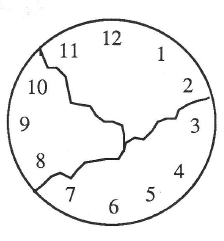
\includegraphics[height=3 cm]{clock}
\end{center}
Assume that each piece has at least two numbers and that no number is damaged (e.g. 12 isn't split into two digits 1 and 2.) 
\end{problem}


\fellow{Replace clock picture as before.}

Remember that your first step is to understand the problem.  Work out what's going on here.  What are the sums of the numbers on each piece?  Are they consecutive?  (What does that mean?)

\begin{thinkpair*}
After you have worked on the problem on your own for a while, talk through your ideas with a partner (even if you haven't solved it).  What did you try?   What progress have you made?
\end{thinkpair*}


\begin{ps}[Find the Math, Remove the Context]
Sometimes the problem has a lot of details in it that are unimportant, or at least unimportant for getting started.  The goal is to find the underlying math problem, then come back to the original question and see if you can solve it using the math.
\end{ps}

In this case, worrying about the clock and exactly how the pieces break is less important than worrying about finding consecutive numbers that sum to the correct total.  Ask yourself: 
\begin{itemize}
\item
What is the sum of all the numbers on the clock's face?  
\item
Can I find two consecutive numbers that give the correct sum?  Or four consecutive numbers?  Or some other amount?
\item
How do I know when I'm done?  When should I stop looking?
\end{itemize}

Of course, solving the question about consecutive numbers is not the same as solving the original problem.  You have to go back and see if the clock can actually break apart so that each piece gives you one of those consecutive numbers.  Maybe you can solve the math problem, but it doesn't translate into solving the clock problem.

\begin{ps}[Check Your Assumptions]
When solving problems, it's easy to limit your thinking by adding extra assumptions that aren't in the problem.  Be sure you ask yourself: Am I constraining my thinking too much?
\end{ps}

In the clock problem, because the first solution has the clock broken \emph{radially} (all three pieces meet at the center, so it looks like slicing a pie), many people assume that's how the clock must break.  But the problem doesn't require the clock to break radially.  It might break into pieces like this:

\fellow{Add a picture of a clock broken into pieces with the breaks going across, not radial.  For example, three pieces: $\{11, 12, 1, 2\}$, $\{10,9, 3, 4, 5\}$, and $\{6,7,8\}$.}


Were you assuming the clock would break in a specific way?  Try to solve the problem now, if you haven't already.  


\section{Beware of Patterns!}\label{sec:BewarePatterns}

The ``Look for Patterns'' strategy can be particularly appealing, but you have to be careful!  Don't forget the {\bf ``and Explain''} part of the strategy.  Not all patterns are obvious, and not all of them will continue.

\begin{problem}[Dots on a Circle]
Start with a circle.  
\begin{center}

\includegraphics[height=3 cm]{circle}
\end{center}
If I put two dots on the circle and connect them, the line divides the circle into two pieces.
\begin{center}
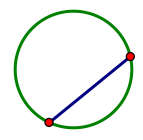
\includegraphics[height=3 cm]{twodots}
\end{center}
If I put three dots on the circle and connect each pair of dots, the lines divides the circle into four pieces.
\begin{center}
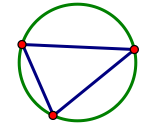
\includegraphics[height=3 cm]{threedots}
\end{center}
Suppose you put one hundred dots on a circle and connect each pair of dots.  How many pieces will you get? 
\end{problem}

\begin{thinkpair*}
After you have worked on the problem on your own for a while, talk through your ideas with a partner (even if you haven't solved it).  What strategies did you try?   What did you figure out?  What questions do you still have?
\end{thinkpair*}


The natural way to work on this problem is to use smaller numbers of dots and look for a pattern, right?  If you haven't already, try it.  How many pieces when you have four dots?  Five dots?   How would you describe the pattern?

Now try six dots.  You'll want to draw a \emph{big} circle and space out the six dots to make your counting easier.  Then carefully count up how many pieces you get.  It's probably a good idea to work with a partner so you can check each other's work.  Make sure you count every piece once and don't count any piece twice.  How can you be sure that you do that?

Were you surprised?  For the first several steps, it  \emph{seems} to be the case that when you add a dot you double the number of pieces.  But that would mean that for six dots, you should get 32 pieces, and you only get 31!  The pattern simply doesn't hold up.


Mathematicians love looking for patterns and finding them.  We get excited by patterns.   But we are also very skeptical of patterns!  If we can't explain \emph{why} a pattern would occur, then we aren't willing to just believe it!  

For example, if my number pattern starts out 
\[
2, 4, 8, \dots
\]
I can find \emph{lots} of ways to continue the pattern, each of which makes sense in some contexts.  Here are some possibilities:
\begin{itemize}
\item
$2, 4, 8, 2, 4, 8, 2, 4, 8, 2, 4, 8, \dots$. \\
This is a a repeating pattern, cycling through the numbers $2, 4, 8$ and then starting over with $2$.\\

\item
$2, 4, 8, 32, 256, 8192,  \dots$. \\
To get the next number, multiply the previous two numbers together.\\

\item
$2, 4, 8, 16, 32, 64, 128, 256, 512, 1024,  \dots$. \\

\item
$2, 4, 8, 14, 22, 32, 44, 58, 74  \dots$. \\

\end{itemize}


\begin{thinkpair*}
Work on your own and then share your ideas with a partner:
\begin{enumerate}
\item
For the last two patterns above, describe in words how the number sequence is being created.  
\item
Find at least two other ways to continue the sequence $2, 4, 8, \dots$ that looks different from all the ones you've seen so far.  Write your rule in words, and write the next five terms of the number sequence.
\end{enumerate}
\end{thinkpair*}

So how can you be sure your pattern fits the problem?  You have to tie them together!  Remember the ``Squares on a Chess Board'' problem?  You might have noticed a pattern like this one:

If the chess board has 5 squares on a side, then there are
\begin{itemize}
\item
$5 \times 5 =25$ squares of size $1 \times 1$.
\item
$4 \times 4 = 16$ squares of size $2 \times 2$.
\item
$3 \times 3 =9$ squares of side $3 \times 3$.
\item 
$2 \times 2 = 4$ squares of size $4 \times 4$.
\item
$1 \times 1 = 1$ squares of size $5 \times 5$.
\end{itemize}
So there are a total of
\[
1^2 + 2^2 + 3^2 + 4^2 + 5^2 = 55
\]
squares on a $5 \times 5$ chess board.

You can probably guess how to continue the pattern to any size board, but  how can you be \emph{absolutely sure} the pattern continues in this way?  What if this is like ``Dots on a Circle,'' and the obvious pattern breaks down after a few steps? You have to tie the pattern to the problem, so that it's clear why the pattern \emph{must} continue in that way.

The first step in explaining a pattern is writing it down clearly.  This brings us to another problem solving strategy.

\begin{ps}[Use a Variable!]
One of the most powerful tools we have   is the use of a \emph{variable}.  If you find yourself doing calculations on things like ``the number of squares,'' or ``the number of dots,'' give those quantities a name!  They become much easier to work with.
\end{ps}

\begin{thinkpair*}
For now, just work on \emph{describing} the pattern with variables.  
\begin{itemize}
\item
Stick with a $5 \times 5 $ chess board for now, and consider a small square of size $k \times k$.  Describe the pattern: How many squares of size $k \times k$ fit on a chess board of size $5\times 5$?
\item
What if the chess board is bigger?  Based on the pattern above,  how many squares of size $k \times k$ \emph{should} fit on a chess board of size $10 \times 10$?
\item
What if you don't know how big the chess board is?  Based on the pattern above,  how many squares of size $k \times k$ \emph{should} fit on a chess board of size $n \times n$?
\end{itemize}
\end{thinkpair*}

Now comes the tough part: \emph{explaining} the pattern.  Let's focus on an $8 \times 8$ board.  Since it measures $8$ squares on each side, we can see that we get $8 \times 8 = 64$ squares of size $1 \times 1$.  And since there's just a single board, we get just one square of size $8 \times 8$.  But what about all the sizes in-between?

\fellow{Insert video showing why the count for $2 \times 2$ squares should be $7 \times 7  = 49$.  Model it on the general solution below.}

\begin{thinkpair*}
Using the video as a model, work with a partner to carefully explain why the number of $3 \times 3$ squares will be $6 \times 6 = 36$, and why the number of $4 \times 4$ squares will be $4 \times 4 = 16$.
\end{thinkpair*} 

Here's what a final justification might look like:  

\begin{sol*}[Chess Board Pattern]
Let $n$ be the side of the chess board and let $k$ be the side of the square.  If the square is going to fit on the chess board at all, it must be true that $k \leq n$.  Otherwise, the square is too big.

If I put the $k \times k$ square in the upper left corner of the chess board, it takes up $k$ spaces across and there are $(n-k)$ spaces to the right of it.  So I can slide the $k \times k$ square to the right $(n-k)$ times, until it hits the top right corner of the chess board.  The square is in $(n-k+1)$ different positions, counting the starting position.

If I move the $k \times k$ square back to the upper left corner, I can shift it down one row and repeat the whole process again.  Since there are $(n-k)$ rows below the square, I can shift it down $(n-k)$ times until it hits the bottom row.  This makes $(n-k+1)$ total rows that the square moves across, counting the top row.

So there are $(n-k+1)$ rows with $(n-k+1)$ squares in each row.  That makes $(n-k+1)^2$ total squares.  
\end{sol*}

Once we're sure the pattern continues, we can use it to solve the problem.  So go ahead!  
\begin{itemize}
\item
How many squares on a $10 \times 10$ chess board?    
\item
What calculation would you do to solve that problem for a $100 \times 100$ chess board?
\end{itemize}


There \emph{is} a number pattern that describes the number of pieces you get from the ``Dots on a Circle'' problem.  If you want to solve the problem, go for it!  Think about all of your problem solving strategies.  But be sure that when you find a pattern, you can explain \emph{why} it's the right pattern for this problem, and not just another pattern that seems to work but might not continue.


\section{Problem Bank}\label{sec:ProblemBank}
You have several problem solving strategies to work with.  Here are the ones we've described in this Section (and you probably came up with even more of your own strategies as you worked on problems).
\begin{enumerate}
\item
Wishful Thinking.
\item
Try Something!
\item
Draw a Picture.
\item
Make up Numbers.
\item
Try a Simpler Problem.
\item
Work Systematically.
\item
Use Manipulatives to Help You Investigate.
\item
Look for and Explain Patterns.
\item
Find the Math, Remove the Context.
\item
Check Your Assumptions.
\item
Use a Variable.
\end{enumerate}

Try your hand at some of these problems, keeping these strategies in mind.  If you're stuck on a problem, come back to this list and ask yourself which of the strategies might help you make some progress.


\fellow{If you have any favorite problems that don't have a lot of mathematical prerequisites --- this is the first chapter! --- throw them in!  The more the merrier!}



\begin{problem}
You have eight coins and a balance scale.  The coins look alike, but one of them is a counterfeit.  The counterfeit coin is lighter than the others.  You may only use the balance scale two times.  How can you find the counterfeit coin?

\fellow{Balance scale picture?}
\end{problem}



\begin{problem}
You have five coins, no two of which weigh the same.  In seven weighings on a balance scale, can you put the coins in order from lightest to heaviest?  That is, can you determine which  coin is the lightest, next lightest, \dots, heaviest.  
\end{problem}

\begin{problem}
You have ten bags of coins.  Nine of the bags contain good coins weighing one ounce each.  One bag contains counterfeit coins weighing 1.1 ounces each.  You have a regular (digital) scale, not a balance scale.  The scale is correct to one-tenth of an ounce.  In one weighing, can you determine which bag contains the bad coins?
\end{problem}

\begin{problem}
Suppose you have a balance scale.  You have three different weights, and you are able to weigh every whole number from 1 gram to 13 grams using just those three weights.  What are the three weights?  
\end{problem}



\begin{problem}
There are a bunch of coins on a table in front of you.  Your friend tells you how many of the coins are heads-up.  You are blindfolded and can't see a thing, but you can move the coins around, and you can flip them over.  However, you can't tell just by feeling them if the coins are showing heads or tails.  Your job: separate the coins into two piles so that the same number of heads are showing in each pile.
\end{problem}


\begin{problem}
The digital root of a number is the number obtained by adding the digits of the number.  If the answer is not a one-digit number, add those digits.  Continue until a one-digit sum is reached.  This one digit is the digital root of the number.  For example, the digital root of 98 is 8, since 
$$
9+8 = 17 \quad \text{and} \quad 1+7 = 8.
$$
Record the digital roots of the first $30$ integers and find as many  patterns as you can.  Can you explain any of the patterns?  Can you predict the digital root of a number without computing it? 
\end{problem}

\begin{problem}
If this lattice were continued, what number would be directly to the right of $98$?
\begin{center}
\begin{tabular}{c c c c c c c c c c c}
& 3 &  & 6 &  & 9 &  & 12 & &\ldots \\
1 & 2& 4&  5 & 7 & 8 & 10 & 11 & 13 & \ldots  \\
\end{tabular}
\end{center}

\end{problem}





\begin{problem}
Arrange the digits $0$ through $9$ so that the first digit is divisible by $1$, the first two digits are divisible by $2$, the first three digits are divisible by $3$, and continuing until you have the first $9$ digits divisible by $9$ and the whole $10$-digit number divisible by~$10$.
\end{problem}

\begin{problem}
There are 25 students and one teacher in class.  After an exam, everyone high-fives everyone else to celebrate how well they did.  How many high-fives were there?
\end{problem}




\begin{problem}
In cleaning out your old desk, you find a whole bunch of $3$\textcent\ and $7$\textcent\ stamps.  Can you make exactly $11$\textcent\ of postage?  Can you make exactly $19$\textcent\ of postage?  What is the largest amount of postage you cannot make?  
\end{problem}


\begin{problem}
Find the largest eight-digit number made up of the digits 1, 1, 2, 2, 3, 3, 4, and 4 such that the 1s are separated by one digit, the 2s are separated by two digits, the 3s by three digits, and the 4s by four digits.
\end{problem}



\begin{problem}
Kami has ten pockets and 44 dollar bills.  She wants to have a different amount of money in each pocket.  Can she do it?
\end{problem}


\begin{problem}
How many triangles are in this picture?
\begin{center}
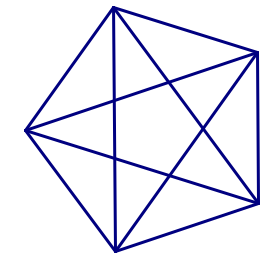
\includegraphics[height=3 cm]{pent_tris}
\end{center}


\end{problem}

\begin{problem}
Arrange the digits 1--6 into a ``difference triangle'' where each number in the row below is the difference of the two numbers above it.\\
{\bf Example:} This is a difference triangle, but it doesn't work because it uses 1 twice and doesn't have a 6:

\begin{center}
\begin{tabular}{c c c c c}
4 && 5 && 3 \\
 & 1 && 2\\
 &&1 \\
 \end{tabular}
 \end{center}
\end{problem}


\begin{problem}
Certain pipes are sold in lengths of 6 inch, 8 inch, and 10 inches.  How many different lengths can you form by attaching three sections of pipe together?
\end{problem}

\begin{problem}
Place the digits 1, 2, 3, 4, 5, 6 in the circles so that the sum on each side of the triangle is 12.  Each circle gets one digit, and each digit is used exactly once.
\begin{center}
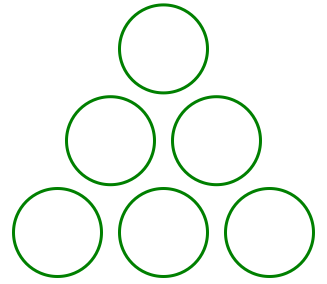
\includegraphics[height=3 cm]{circle_pyr}
\end{center}

\end{problem}


\begin{problem}
Find a way to cut a circular pizza into 11 pieces using just four straight cuts.
\end{problem}



\section{Careful use of Language in Mathematics}
This section might seem like a bit of a sidetrack from the idea of problem solving, but in fact it's not.  Mathematics is a social endeavor.  We don't just solve problems and then put them aside.  Problem solving has (at least) three components:
\begin{enumerate}
\item
Solving the problem.  This involves lots of scratch paper and careful thinking.
\item
Convincing \emph{yourself} that your solution is complete and correct.  This involves a lot of self-check and asking yourself questions.
\item
Convincing \emph{someone else} that your solution is complete and correct.  This usually involves writing the problem up carefully or explaining your work in a presentation.
\end{enumerate}

If you're not able to do that last step, then you haven't really solved the problem.  We'll talk more about how to write up a solution in the next section.  Before we do that, we have to think about how mathematicians use language (which is, it turns out, a bit different from how language is used in the rest of life).

\subsection{Mathematical Statements}

\begin{define}
A {\bf mathematical statement} is a complete sentence that is either true or false.
\end{define}

So a ``statement'' in mathematics cannot be a question, a command, or a matter of opinion.  It is a complete, grammatically correct sentence (with a subject, verb, and usually an object).  It's important that the statement is either true or false, though you may not know which!  (Part of the work of a mathematician is figuring out which sentences are true and which are false.

\begin{thinkpair*}
For each English sentence below, decide if it is a mathematical statement or not.  If it is, is the statement true or false (or are you unsure)?  If it is not, in what way does it fail?

\begin{enumerate}
\item
I like the color blue.
\item
$60$ is an even number.
\item
Is your dog friendly?
\item
Honolulu is the capital of Hawaii.
\item
This sentence is false.
\item
Roses are red.
\item
UH Manoa is the best college in the world.
\item
$1/2 = 2/4$.
\item
Go to bed.
\item
There are a total of 204 squares on an $8 \times 8$ chess board.
\end{enumerate}

Now, work with a partner.  Write three mathematical statements and three English sentences that fail to be mathematical statements.
\end{thinkpair*}

Notice that ``$1/2 = 2/4$'' is a perfectly good mathematical statement.  It doesn't look like an English sentence, but read it out loud.  The subject is ``$1/2$.'' The verb is ``equals.''  And the object is ``$2/4$.''  This is a very good test when you write mathematics: try to read it out loud.  Even the equations should read naturally, like English sentences. 

Statement (5) is different from the others.  It is called a \emph{paradox}: a statement that is self-contradictory.  If it is true, then we conclude that it is false.  (Why?)  If it is false, then we conclude that it is true.  (Why?)  Paradoxes are no good as mathematical statements.  

\subsection{Precision}
When we use words in an everyday situation, we often rely on context and shared understanding.
The American Academy of Dermatology has this sentence on their web page: 
\begin{center}
``One American dies of melanoma every hour.''
\end{center}

Taken literally (as a mathematician would), this statement makes an absurd claim:  There is one person in America who keeps dying over and over.  In fact, he dies \emph{every single hour}.

A more precise statement would be this:
``Every hour, someone in America dies of melanoma.''

\begin{thinkpair*}
Compare the two sentences:
\begin{itemize}
\item
``One American dies of melanoma every hour.''
\item
``Every hour, someone in America dies of melanoma.''
\end{itemize}
What is the (subtle) difference?  Why does that small difference change the meaning so dramatically?

\end{thinkpair*}

 If we're working on mathematical problem, we need to work with clear and correct statements.  We cannot make assumptions about context or shared understanding.  We have to say exactly what we mean.

\subsection*{On Your Own}
Work on the exercises below to reinforce the idea of using precise language.
\begin{enumerate}
\item
Consider this ambiguous sentence:
\begin{center}
\emph{``The man saw
the woman with a telescope.''} 
\end{center}
Find two unambiguous (but natural sounding) sentences equivalent to the sentence above, one in which the
 man has the telescope, and one in which  the woman
has the telescope.
 
 
 \item
Here are three ambiguous newspaper headlines.  For each one, rewrite it in a way that avoids the unintended second meaning.  But keep it short and pithy, like a newspaper headline should be.

\begin{enumerate}
\item
Sisters reunited after 10 years in checkout line of Longs Drugs.
\item
Large hole appears on H-1.  County authorities are looking into it.
\item
Governor Abercrombie says bus passengers should be belted.

\end{enumerate}


 \item
This hospital notice says exactly the opposite of what it means to say.
 \begin{center}
\emph{``No head injury is too trivial to ignore.''} 
\end{center}
Rewrite the sentence so it would still fit on the sign, but would convey its intended meaning.



\end{enumerate}


\subsection{And / or}
Consider this sentence 
\begin{center}
\emph{``After work, I will go to the beach or I will do my grocery shopping.''}
\end{center}
In everyday English, that probably means that if I go to the beach, I will not go shopping.  I will do one or the other, but not both activities.  This is called an ``exclusive or.''

We can usually tell from context whether a speaker means ``either one or the other or both,'' or whether he means ``either one or the other but not both.''  (Some people use the awkward phrase ``and/or'' to describe the first option.)  

Remember that in mathematical communication, though, we have to be very precise.  We cannot rely on context or assumptions about what is implied or understood.
\begin{define}
In mathematics, the word ``or'' \emph{always means} ``either one or the other or both.''
\end{define}

\begin{thinkpair*}
For each sentence below:
\begin{itemize}
\item
Decide if the choice $x = 3$ makes the statement true or false.  
\item
Choose a different value of $x$ that makes the statement true (or say why that's not possible).
\item
Choose a different value of $x$ that makes the statement false (or say why that's not possible).
\end{itemize}

\begin{enumerate}
\item
$x$ is odd or $x$ is even.
\item
$x$ is odd and $x$ is even.
\item
$x$ is prime or $x$ is negative.
\item
$x >5$ or $x < 5$.
\item
$x >5$ and $x < 5$.
\item
$x + 1 = 7$ or $x - 1 = 7$.
\item
$x \cdot 1 = x$ or $x \cdot 0 = x$.
\item
$x \cdot 1 = x$ and $x \cdot 0 = x$.
\end{enumerate}
\end{thinkpair*}



\subsection{Quantifiers}
\begin{problem}[All About the Benjamins]
You are handed an envelope filled with money, and you are told ``Every bill in this envelope is a \$100 bill.''
\begin{itemize}
\item
What would convince you \emph{beyond any doubt} that the sentence is true?  How could you convince someone else that the sentence is true?

\item 
What would convince you \emph{beyond any doubt} that the sentence is false?  How could you convince someone else that the sentence is false?
\end{itemize}

Suppose you were given a different sentence: ``There is a \$100 bill in this envelope.''
\begin{itemize}
\item
What would convince you \emph{beyond any doubt} that the sentence is true?  How could you convince someone else that the sentence is true?

\item 
What would convince you \emph{beyond any doubt} that the sentence is false?  How could you convince someone else that the sentence is false?
\end{itemize}
\end{problem}

\begin{thinkpair*}
After you have thought about the problem on your own for a while, talk through your ideas with a partner.  What is the difference between the two sentences?  How does that difference affect your method to decide if the statement is true or false?
\end{thinkpair*}

Some mathematical statements have this form:
\begin{itemize}
\item
``Every time\dots''
\item
``For all numbers\dots''
\item
``For every choice\dots''
\item
``It's always true that\dots''
\end{itemize} 
These are \emph{universal statements}.  Such statements claim that something is always true, no matter what.  

\begin{itemize}
\item
To prove a \emph{universal statement} is false, you must find an example where it fails.  This is called a {\bf counterexample} to the statement.
\item
To prove a \emph{universal statement} is true, you must either check every single case, or you must find a {\bf logical reason} why it would be true.  (Sometimes the first option is impossible, because there might be infinitely many cases to check.  You would never finish!)
\end{itemize}


Some mathematical statements have this form:
\begin{itemize}
\item
``Sometimes\dots''
\item
``There is some number\dots''
\item
``For some choice\dots''
\item
``At least once\dots''
\end{itemize} 
These are \emph{existential statements}.  Such statements claim there is some example where the statement  is  true, but it may not always be true.  

\begin{itemize}
\item
To prove an \emph{existential statement} is true, you may just find the example where it works.  
\item
To prove an \emph{existential statement} is false, you must either show it fails in every single case, or you must find a {\bf logical reason} why it can't be true.  (Sometimes the first option is impossible!)
\end{itemize}



\begin{thinkpair*}
For each statement below, do the following:
\begin{itemize}
\item
Decide if it is a \emph{universal statement} or an \emph{existential statement}.  (This can be tricky because in some statements the quantifier is ``hidden'' in the meaning of the words.)
\item
Decide if the statement is true or false, and do your best to justify your decision.
\end{itemize}

\begin{enumerate}
\item
Every odd number is prime.
\item
Every prime number is odd.
\item
For all positive numbers $x$, $x^3 > x$.
\item
There is some number $x$ such that $x^3 = x$.
\item
The points $(-1,1)$, $(2,1)$, and $(3,0)$ all lie on the same line.
\item
Addition (of real numbers) is commutative.
\item
Division (of real numbers) is commutative.
\end{enumerate}

Look back over your work.  you will probably find that some of your arguments are sound and convincing while others are less so.  In some cases you may ``know'' the answer but be unable to justify it.  That's okay for now!  Divide your answers into four categories:

\bigskip

\begin{enumerate}[(a)]
\item
I am confident that the justification I gave is good.
\item
I am not confident in the justification I gave.
\item
I am confident that the justification I gave is \emph{not} good, or I could not give a justification.
\item
I could not decide if the statement was true or false.
\end{enumerate}


\end{thinkpair*}

\subsection{Conditional statements}
\begin{problem}[Card Logic]
These cards are on a table.
\begin{center}
\includegraphics[height=3 cm]{cards}
\end{center}
Your friend claims: ``If a card has a vowel on one side, then it has an even number on the other side.'' Which cards \emph{must} you flip over to  be certain that your friend is telling the truth?
\end{problem}


\fellow{Picture is stolen from a long-forgotten source.  Can we re-create it so it's not any kind of copyright violation?}


\begin{thinkpair*}
After you have thought about the problem on your own for a while, discuss your ideas with a partner.  Do you agree on which cards you must check?   Try to come to agreement on an answer you both believe.
\end{thinkpair*}

Here is another very similar problem, yet people seem to have an easier time solving this one:


\begin{problem}[IDs at a Party]
You are in charge of a party where there are young people. Some are drinking alcohol, others soft
drinks. Some are old enough to drink alcohol legally, others are under age. You are responsible for
ensuring that the drinking laws are not broken, so you have asked each person to put his or her
photo ID on the table. At one table, there are four young people:
\begin{itemize}
\item
One person has a beer, another has a
Coke, but their IDs happen to be face down so you cannot see their ages. 
\item
You can, however, see the
IDs of the other two people. One is under the drinking age, the other is above it. Unfortunately,
you are not sure if they are drinking Seven-up or vodka and tonic. 
\end{itemize}
Which IDs and/or drinks do you
need to check to make sure that no one is breaking the law?
\end{problem}

\begin{thinkpair*}
After you have thought about the problem on your own for a while, discuss your ideas with a partner.  Do you agree on which cards you must check?   Compare these two problems.
Which question is easier and why?
\end{thinkpair*}

\begin{define}
A {\bf conditional statement} can be written in the form
\begin{center}
If $\underbrace{\quad \text{\emph{some statement}} \quad}_{\text{hypothesis}}$ then $\underbrace{\quad \text{\emph{some statement}}  \quad}_{\text{conclusion}}$.
\end{center}
\end{define}

\begin{thinkpair*}
 These are each conditional statements, though they are not all stated in ``if/then'' form.  Identify the hypothesis of each statement.  (You may want to rewrite the sentence as an equivalent ``if/then'' statement.)
 \vspace{.2in}

 \begin{enumerate}
\item 
If the tomatoes are red, then they are ready to eat.\\
The tomatoes are red. \qquad / \qquad The tomatoes are ready to eat.


\item
An integer $n$ is even if it is a multiple of 2.\\
$n$ is even. \qquad / \qquad $n$ is a multiple of 2.



\item
If $2^n - 1$ is prime, then $n$ is prime.\\
$n$ is prime. \qquad / \qquad $2^n-1$ is prime.



\item
The team wins when JJ plays.\\
The team wins. \qquad / \qquad JJ plays.


\end{enumerate}
\end{thinkpair*}

Remember that a mathematical statement must have a definite truth value.  It's either true or false, with no gray area (even though we may not be sure which is the case).  How can you tell if a conditional statement is true or false?  Surely, it depends on whether the \emph{hypothesis} and the \emph{conclusion} are true or false.  But how, exactly, can you decide?

The key is to think of a conditional statement like a promise, and ask yourself: under what condition(s) will I have broken my promise?

\begin{example}
Here is a conditional statement:
\begin{center}
``If $\underbrace{\text{I win the lottery}}_{\text{hypothesis}}$, then $\underbrace{\text{I'll give  each of my students \$1,000}}_{\text{conclusion}}$.''
\end{center}

There are four things that can happen:
\begin{description}
\item[True hypothesis, true conclusion] I do win the lottery, and I do give everyone in class \$1,000.   I kept my promise, so the conditional statement is TRUE.
\item[True hypothesis, false conclusion] I do win the lottery, but I decide {\bf not to} give everyone in class \$1,000.   I broke my promise, so the conditional statement is FALSE.
\item[False hypothesis, true conclusion] I don't win the lottery, but I'm exceedingly generous, so I go ahead and give everyone in class \$1,000.  I didn't break my promise!  (Do you see why?)  So the conditional statement is TRUE.
\item[False hypothesis, false conclusion] I don't win the lottery,  so I don't give everyone in class \$1,000.  I didn't break my promise!  (Do you see why?)  So the conditional statement is TRUE.
\end{description}
\end{example}

What can we conclude from this?  {\bf A conditional statement is false only when the hypothesis is true and the conclusion is false.}  In every other instance, the promise (as it were) has not been broken.  If the statement is not false, it must be true.

\begin{example}
Here's another conditional statement:
\begin{center}
``If you live in Honolulu, then you live in Hawaii.''
\end{center}
Is this statement true or false?  It seems like it should depend on who the pronoun ``you'' refers to, and whether that person lives in Honolulu or not.  Let's think it through:
\begin{itemize}
\item
Sookim lives in Honolulu, so the hypothesis is true.  Since Honolulu is in Hawaii, she does live in Hawaii.  The statement is true about Sookim, since both the hypothesis and conclusion are true.
\item
DeeDee lives in Los Angeles.  The statement is true about DeeDee since the hypothesis is false.
\end{itemize} 

So in fact it doesn't matter!  The statement is true either way.  The right way to understand such a statement is as a \emph{universal statement}: ``Everyone who lives in Honolulu lives in Hawaii.''  

This statement is true, and here's how you might justify it:  ``Pick a random person who lives in Honolulu.  That person lives in Hawaii (since Honolulu is in Hawaii), so the statement is true for that person.  I don't need to consider people who don't live in Honolulu.  The statement is \emph{automatically} true for those people, because the hypothesis is false!''
\end{example}

\begin{example}
How do we show a (universal) conditional statement is false?  You need to give a specific instance where the hypothesis is true and the conclusion is false.  For example:
\begin{center}
``If you are a good swimmer, then you are a good surfer.''
\end{center}
Do you know someone for whom the hypothesis is true (that person is a good swimmer) but the conclusion is false (the person is not a good surfer)?  Then the statement is false!
\end{example}

\begin{thinkpair*}
For each conditional statement, decide if it is true or false.  Justify your answer.  
\begin{enumerate}
\item
If $2 \times 2 = 4$ then $1 + 1 = 3$.

\item
If $2 \times 2 = 5$ then $1 + 1 = 3$.


\item
If $\pi > 3$ then all odd numbers are prime.

 \item
If $\pi < 3$ then all odd numbers are prime.


\item
If the units digit of a number is 4, then the number is even.

\item
If a number is even, then the units digit of that number is 4.

\item
If the product of two numbers is 0, then one of the numbers is 0.

\item
If the sum of two numbers is 0, then one of the numbers is 0.

\item
If you are tall, then you have long hair.



\end{enumerate}
\end{thinkpair*}


\begin{thinkpair*}[Two truths and a lie]
On your own, come up with two conditional statements that are true and one that is false.  Share your three statements with a partner, but don't say which are true and which is false.  See if your partner can figure it out!
\end{thinkpair*}



\section{Explaining Your Work}
At its heart, mathematics is a social endeavor.  Even if you work on problems all by yourself, you haven't really \emph{solved} the problem until you've explained your work to someone else, and they sign off on it.  Professional mathematicians write journal articles, books, and grant proposals.  Teachers explain mathematical ideas to their students both in writing and orally.  
Explaining your work is really an essential part of the problem-solving process, and probably should have been Polya's step (5).

Writing in mathematics is different from writing poetry or an English paper.  The goal of mathematical writing is not florid description, but clarity.  If your reader doesn't understand, you haven't done a good job.  Here are some tips for good mathematical writing.

\begin{description}
\item[Don't Turn in Scratch Work] When you are solving \emph{problems} and not \emph{exercises}, you're going to have lots of false starts.  You're going to try lots of things that don't work.  You're going to make lots of mistakes.  You're going to use scratch paper.  At some point (hopefully!) you will scribble down an idea that actually solves the problem.  Hooray!  That paper is \emph{not} what you want to turn in or share with the world.  Take that idea, and write it up carefully, neatly, and clearly.  (The rest of these tips apply to that write-up.)

\item[(Re)state the Problem]  Don't assume your reader (even if it's the teacher who assigned the problem!) knows what problem you're solving.  If the problem has a very long description, you can summarize it.  You don't have  rewrite it word-for-word or  give all of the details.  But make sure the question  is clear.

\item[Clearly Give the Answer] It's not a bad idea to state the answer right up front, then show the work to justify your answer.  That way, the reader knows what you're trying to justify as they read.  It makes their job much easier, and making the reader's job easier should be one of your primary goals!  In any case, the answer should be \emph{clearly} stated somewhere in the writeup, and it should be easy to find. 

\item[Be Correct] Of course, everyone makes mistakes as they're working on a problem.  But we're talking about after you've solved the problem, when you are writing up your solution to share with someone else.
The best writing in the world can't save a wrong approach and a wrong answer.  Check your work carefully.  Ask someone else to read your solution with a critical eye.  

\item[Justify Your Answer] You cannot simply give an answer and expect your reader to ``take your word for it.'' You have to explain how you know your answer is correct.  This means ``showing your work,'' explaining your reasoning, and justifying what you say.   You need to answer the question, ``How do you \emph{know} your answer is right?''

\item[Be Concise] There is no bonus prize for writing a lot in math class.  Think clearly and write clearly.  If you find yourself going on and on, stop, think about what you really want to say, and start over.


\item[Use Variables and Equations] Often an equation is much easier to read and understand (and is more concise!) than a long paragraph of text describing a calculation.  Mathematical writing often has way fewer words (and way more equations) than other kinds of writing.

\item[Define your Variables] If you use variables or equations in the solution of your problem, always say what the variable stands for \emph{before} you use it.  If you use an equation, say where it comes from and why it applies to this situation.  Don't make your reader guess!

\item[Use Pictures] If pictures helped you solve the problem, include those pictures in your final solution.  Even if you didn't draw a picture to solve the problem, it still might help your reader understand the solution.  And that's your goal!

\item[Use Correct Spelling and Grammar] Proofread your work.  A good test is to read your work aloud.  There should be complete, natural-sounding sentences.  This includes reading the equations and calculations aloud.  They should read naturally and make sense.   Be especially careful with pronouns.  Avoid using ``it'' and ``they'' for mathematical objects; use the names of the objects (or variables) instead.

\item[Format Clearly] Don't write one long paragraph.  Separate your thoughts.   Put complicated equations on a single displayed line rather than in the middle of a paragraph.  Don't write too small.  Don't make your reader struggle to read and understand your work.

\item[Acknowledge Collaborators] If you worked with someone else on solving the problem, give them credit!


\end{description}

Here is a problem you've already seen:
\begin{problem*}
Find the largest eight-digit number made up of the digits 1, 1, 2, 2, 3, 3, 4, and 4 such that the 1s are separated by one digit, the 2s are separated by two digits, the 3s by three digits, and the 4s by four digits.

\end{problem*}

\begin{thinkpair*}
Below you will find several solutions that were turned in by students.  Using the criteria above, how would you score these solutions on a scale of 1 to 5?  Give reasons for your answers.
\end{thinkpair*}

\begin{sol*}[Solution 1]
41312432


This is the largest eight-digit b/c  the \#s 1, 2, 3, 4 \& all separated by the given amount of spaces.

\end{sol*}


\begin{sol*}[Solution 2]
41312432


You have to have the 4 in the highest place and work down from there.  However unable to follow the rules the 2 and the 1 in the 10k and 100k place must switch.

\end{sol*}


\begin{sol*}[Solution 3]
41312432


First, I had to start with the \#4 because that is the largest digit I could start with to get the largest \#.



Then I had to place the next 4 five spaces away because I knew there had to be four digits separating the two 4s.


Next, I place 1 in the second digit spot because 2 or 3 would interfere with the rule of how many digits could separate them, which allowed me to also place where the next 1 should be.


I then placed the 3 because opening spaces showed me that I could fit three digits in between the two 3s.


Lastly, I had to input the final 2s, which worked out because there were two digits separating them.

\end{sol*}


\begin{sol*}[Solution 4]\ 

1x1\\

2xx2\\

3xxx3\\

4xxxx4



Answer: 41312432

\end{sol*}


\begin{sol*}[Solution 5]
\[
\underline{4} \ \underline{3} \ \underline{\ } \ \underline{2}\  \underline{4}\ \underline{3} \ \underline{2} \ \underline{\ }
\]
\[
\underline{4} \ \underline{2} \ \underline{\ } \ \underline{\ }\  \underline{2}\ \underline{4} \ \underline{\ } \ \underline{\ }
\]
\[
\underline{4} \ \underline{\ } \ \underline{1} \ \underline{3}\  \underline{1}\ \underline{4} \ \underline{\ } \ \underline{3 }
\]
\[
\star \underline{4} \ \underline{1} \ \underline{ 3} \ \underline{1}\  \underline{2}\ \underline{4} \ \underline{3} \ \underline{2}
\]



4 needs to be the first \# to make it the biggest.  Then check going down from next largest to smallest.  Ex:
\[
\underline{4} \ \underline{3} \ \underline{\qquad \qquad \qquad  } \times
\]

\[
\underline{4} \ \underline{2} \ \underline{\qquad \qquad \qquad  } \times
\]

\[
\underline{4} \ \underline{1} \ \underline{\qquad \qquad \qquad  } \checkmark
\]

\end{sol*}


\begin{sol*}[Solution 6]
41312432



I put 4 at the 10,000,000 place because the largest \# should be placed at the highest value.




Numbers 2 \& 3 could not be placed in the 1,000,000 place because I wasn't able to separate the digits properly.




So I ended up placing the \#1 there.  In the 100,000 place I put the \#3 because it was the second higehst number.

\end{sol*}



\begin{sol*}[Solution 7]

41312432



Since the problem asks you for the largest 8 digit \#, I knew 4 had to be the first \# since it's the greatest \# of the set.





To solve the rest of the problem, I used the guess and test method.  I tried many different combinations.  First using the \#3 as the second digit in the sequence, but came to no answer.  Then the \#~2, but no combination I found  correctly finished the sequence.



I then finished with the \#1 in the second digit in the sequence and was able to successfully fill out the entire \#.

\end{sol*}




\begin{sol*}[Solution 8]\ 

$\underline{4} \ \underline{\ } \ \underline{\ } \ \underline{\ }\  \underline{\ }\  \underline{4} \ \underline{\ } \ \underline{\ }$

4 has to be the first digit, for the number to be the largest possible.  That means the other 4 has to be the 6th digit in the number, because 4s have to be separated by four digits.




$\underline{4} \ \underline{\ } \ \underline{3} \ \underline{\ }\  \underline{\ } \ \underline{4}  \ \underline{3 } \ \underline{\ }$

3 must be the third digit, in order for the number to be largest possible.  3 cannot be the second digit because the other 3 would have to be the 6th digit in the number, but 4 is already there.




$\underline{4} \ \underline{1} \ \underline{3} \ \underline{1 }\  \underline{\ } \  \underline{4}\   \ \underline{3 } \ \underline{\ }$

1s must be separated by one digit, so the 1s can only be the 2nd and 4th digit in the number.


$\underline{4} \ \underline{1} \ \underline{3} \ \underline{1 }\  \underline{2} \  \underline{4}\   \ \underline{3 } \ \underline{2 }$

This leaves the 2s to be the 5th and 8th digits.


\end{sol*}


\begin{sol*}[Solution 9]

With the active rules, I tried putting the highest numbers as far left as possible.  Through trying different combinations, I figured out that no two consecutive numbers can be touching in the first two digits.  So I instead tried starting with the 4 then 1 then 3, since I'm going for the highest \# possible.



My answer: 41312432


\end{sol*}


\section{The Last Step}
A lot of people --- from Polya to the writers of the Common Core State Standards and lots of people in between --- talk about problem solving in mathematics.  One fact is rarely acknowledged, except by many professional mathematicians: Asking good questions is as valuable (and as difficult) as solving mathematical problems.  

After solving a mathematical problem and explaining your solution to someone else, it is a very good mathematical habit to ask yourself: What other questions can I ask?

\begin{example}
Recall Problem~\ref{prob:chessboard}, ``Squares on a Chess Board'':

\begin{quote}
How many squares are on a standard $8 \times 8$ chess board?  (The answer is \emph{not} 64!  It's a lot bigger!)
\end{quote}

We've already talked about some obvious follow-up questions like ``What about a $10 \times 10$ chess board?  Or $100 \times 100$?  Or $n \times n$?''

But there are lots of interesting (and less obvious \dots and harder) questions you might ask:
\begin{itemize}
\item
How many \emph{rectangles} can you find on a standard $8 \times 8$ chess board?  (This is a lot harder, because the rectangles come in all different sizes, like $1 \times 2$ and $5 \times 3$.  How could you possibly count them all?)
\item
How many triangles can you find in this picture?
\begin{center}
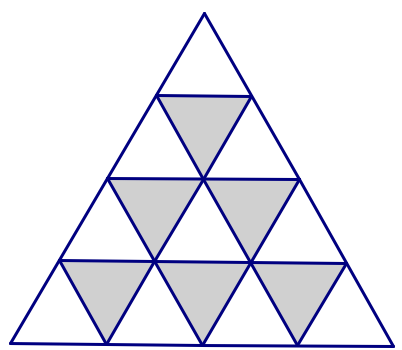
\includegraphics[height=4 cm]{triangleboard}
\end{center}

\end{itemize}

\end{example}

\begin{example}
Recall Problem~\ref{prob:BrokenClock}, ``Squares on a Chess Board'':

\begin{quote}
 This clock has been broken into three pieces.  If you add the numbers in each piece, the sums are consecutive numbers.  Can you break another clock into a different number of pieces so that the sums are consecutive numbers?  
 \begin{center}
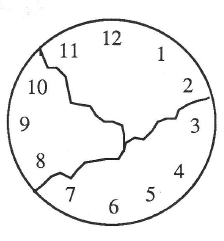
\includegraphics[height=3 cm]{clock}
\end{center}

\end{quote}

The original problem only asks if you can find \emph{one} other way.  The obvious follow-up question: ``Find every possibly way to break the clock into some number of pieces so that the sums of the numbers on each piece are consecutive numbers.  Justify that you have found every possibility.'' 
\end{example}


\begin{thinkpair*}
Choose a problem from the Problem Bank in Section~\ref{sec:ProblemBank} (preferably a problem you have worked on, but that's not strictly necessary).  What follow-up or similar questions could you ask?

\end{thinkpair*}



  
